Suppose you need to implement a special-purpose learning algorithm
that is not included in WEKA. Or suppose you are engaged in machine
learning research and want to investigate a new learning scheme. Or
suppose you just want to learn more about the inner workings of an
induction algorithm by actually programming it yourself. This section
uses a simple example to show how to make full use of WEKA's class
hierarchy when writing classifiers.

\begin{table}[!th]
\footnotesize
{\centering \begin{tabular}{llc}
\hline
Scheme & Description & Book section \\
\hline
\textit{weka.classifiers.bayes.NaiveBayesSimple} & Probabilistic learner & 4.2 \\
\textit{weka.classifiers.trees.Id3} & Decision tree learner & 4.3 \\
\textit{weka.cassifiers.rules.Prism} & Rule learner & 4.4 \\
\textit{weka.classifiers.lazy.IB1} & Instance-based learner & 4.7 \\
\hline
\end{tabular} \footnotesize \par}
\caption{\label{table:simple_schemes}Simple learning schemes in WEKA}
\end{table}


The plugin package called \textit{simpleEducationalLearningSchemes}
includes the elementary learning schemes listed in
Table~\ref{table:simple_schemes}. None take any scheme-specific
command-line options. They are all useful for understanding the inner
workings of a classifier. As an example, we describe
the \textit{weka.classifiers.trees.Id3} scheme, which implements
the \textit{ID3} decision tree learner. Other schemes, such as
clustering algorithms and association rule learners, are organized in
a similar manner.

\section{An example classifier}

\begin{figure}[!thp]
%\centering
\begin{mdframed}[innermargin=-1cm]
\begin{Verbatim}[fontsize=\scriptsize]
import weka.classifiers.*;
import weka.core.*
import java.util.Enumeration;

/**
 * Class implementing an Id3 decision tree learner
 */
public class Id3 extends AbstractClassifier implements TechnicalInformationHandler, Sourcable {

  /** for serialization */
  static final long serialVersionUID = -2693678647096322561L;

  /** The node's successors. */
  private Id3[] m_Successors;

  /** Attribute used for splitting. */
  private Attribute m_Attribute;

  /** Class value if node is leaf. */
  private double m_ClassValue;

  /** Class distribution if node is leaf. */
  private double[] m_Distribution;

  /** Class attribute of dataset. */
  private Attribute m_ClassAttribute;

  /**
   * Returns a string describing the classifier.
   * 
   * @return a description suitable for the GUI.
   */
  public String globalInfo() {
    return "Class for constructing an unpruned decision tree based on the ID3 "
      + "algorithm. Can only deal with nominal attributes. No missing values "
      + "allowed. Empty leaves may result in unclassified instances. For more "
      + "information see: \n\n" + getTechnicalInformation().toString();
  }

  /**
   * Returns an instance of a TechnicalInformation object, containing detailed
   * information about the technical background of this class, e.g., paper
   * reference or book this class is based on.
   * 
   * @return the technical information about this class
   */
  @Override
  public TechnicalInformation getTechnicalInformation() {
    TechnicalInformation result = new TechnicalInformation(Type.ARTICLE);
    result.setValue(Field.AUTHOR, "R. Quinlan");
    result.setValue(Field.YEAR, "1986");
    result.setValue(Field.TITLE, "Induction of decision trees");
    result.setValue(Field.JOURNAL, "Machine Learning");
    result.setValue(Field.VOLUME, "1");
    result.setValue(Field.NUMBER, "1");
    result.setValue(Field.PAGES, "81-106");
    return result;
  }

  /**
   * Returns default capabilities of the classifier.
   * 
   * @return the capabilities of this classifier
   */
  @Override
  public Capabilities getCapabilities() {
    Capabilities result = super.getCapabilities();
    result.disableAll();

    // attributes
    result.enable(Capability.NOMINAL_ATTRIBUTES);

    // class
    result.enable(Capability.NOMINAL_CLASS);
    result.enable(Capability.MISSING_CLASS_VALUES);

    // instances
    result.setMinimumNumberInstances(0);

    return result;
  }
\end{Verbatim}
\end{mdframed}
\caption{\label{fig:scheme_id3}The source code for the \textit{ID3} decision tree learner.}
\end{figure}

\begin{figure}[!thp]
\ContinuedFloat
%\centering
\begin{mdframed}[innermargin=-1cm]
\begin{Verbatim}[fontsize=\scriptsize]
  /**
   * Builds Id3 decision tree classifier.
   * 
   * @param data the training data
   * @exception Exception if classifier can't be built successfully
   */
  @Override
  public void buildClassifier(Instances data) throws Exception {

    // can classifier handle the data?
    getCapabilities().testWithFail(data);

    // remove instances with missing class
    data = new Instances(data);
    data.deleteWithMissingClass();

    makeTree(data);
  }

  /**
   * Method for building an Id3 tree.
   * 
   * @param data the training data
   * @exception Exception if decision tree can't be built successfully
   */
  private void makeTree(Instances data) throws Exception {

    // Check if no instances have reached this node.
    if (data.numInstances() == 0) {
      m_Attribute = null;
      m_ClassValue = Utils.missingValue();
      m_Distribution = new double[data.numClasses()];
      return;
    }

    // Compute attribute with maximum information gain.
    double[] infoGains = new double[data.numAttributes()];
    Enumeration<Attribute> attEnum = data.enumerateAttributes();
    while (attEnum.hasMoreElements()) {
      Attribute att = attEnum.nextElement();
      infoGains[att.index()] = computeInfoGain(data, att);
    }
    m_Attribute = data.attribute(Utils.maxIndex(infoGains));

    // Make leaf if information gain is zero.
    // Otherwise create successors.
    if (Utils.eq(infoGains[m_Attribute.index()], 0)) {
      m_Attribute = null;
      m_Distribution = new double[data.numClasses()];
      Enumeration<Instance> instEnum = data.enumerateInstances();
      while (instEnum.hasMoreElements()) {
        Instance inst = instEnum.nextElement();
        m_Distribution[(int) inst.classValue()]++;
      }
      Utils.normalize(m_Distribution);
      m_ClassValue = Utils.maxIndex(m_Distribution);
      m_ClassAttribute = data.classAttribute();
    } else {
      Instances[] splitData = splitData(data, m_Attribute);
      m_Successors = new Id3[m_Attribute.numValues()];
      for (int j = 0; j < m_Attribute.numValues(); j++) {
        m_Successors[j] = new Id3();
        m_Successors[j].makeTree(splitData[j]);
      }
    }
  }  
\end{Verbatim}
\end{mdframed}
\caption{\label{fig:scheme_id3}The source code for the \textit{ID3} decision tree learner cont.}
\end{figure}

\begin{figure}[!thp]
\ContinuedFloat
%\centering
\begin{mdframed}[innermargin=-1cm]
\begin{Verbatim}[fontsize=\scriptsize]
  /**
   * Classifies a given test instance using the decision tree.
   * 
   * @param instance the instance to be classified
   * @return the classification
   * @throws NoSupportForMissingValuesException if instance has missing values
   */
  @Override
  public double classifyInstance(Instance instance)
    throws NoSupportForMissingValuesException {

    if (instance.hasMissingValue()) {
      throw new NoSupportForMissingValuesException("Id3: no missing values, "
        + "please.");
    }
    if (m_Attribute == null) {
      return m_ClassValue;
    } else {
      return m_Successors[(int) instance.value(m_Attribute)]
        .classifyInstance(instance);
    }
  }

  /**
   * Computes class distribution for instance using decision tree.
   * 
   * @param instance the instance for which distribution is to be computed
   * @return the class distribution for the given instance
   * @throws NoSupportForMissingValuesException if instance has missing values
   */
  @Override
  public double[] distributionForInstance(Instance instance)
    throws NoSupportForMissingValuesException {

    if (instance.hasMissingValue()) {
      throw new NoSupportForMissingValuesException("Id3: no missing values, "
        + "please.");
    }
    if (m_Attribute == null) {
      return m_Distribution;
    } else {
      return m_Successors[(int) instance.value(m_Attribute)]
        .distributionForInstance(instance);
    }
  }

  /**
   * Prints the decision tree using the private toString method from below.
   * 
   * @return a textual description of the classifier
   */
  @Override
  public String toString() {

    if ((m_Distribution == null) && (m_Successors == null)) {
      return "Id3: No model built yet.";
    }
    return "Id3\n\n" + toString(0);
  }

  /**
   * Computes information gain for an attribute.
   * 
   * @param data the data for which info gain is to be computed
   * @param att the attribute
   * @return the information gain for the given attribute and data
   * @throws Exception if computation fails
   */
  private double computeInfoGain(Instances data, Attribute att)
    throws Exception {

    double infoGain = computeEntropy(data);
    Instances[] splitData = splitData(data, att);
    for (int j = 0; j < att.numValues(); j++) {
      if (splitData[j].numInstances() > 0) {
        infoGain -= ((double) splitData[j].numInstances() / (double) data
          .numInstances()) * computeEntropy(splitData[j]);
      }
    }
    return infoGain;
  }
\end{Verbatim}
\end{mdframed}
\caption{\label{fig:scheme_id3}The source code for the \textit{ID3} decision tree learner cont.}
\end{figure}

\begin{figure}[!thp]
\ContinuedFloat
%\centering
\begin{mdframed}[innermargin=-1cm]
\begin{Verbatim}[fontsize=\scriptsize]
  /**
   * Computes the entropy of a dataset.
   * 
   * @param data the data for which entropy is to be computed
   * @return the entropy of the data's class distribution
   * @throws Exception if computation fails
   */
  private double computeEntropy(Instances data) throws Exception {

    double[] classCounts = new double[data.numClasses()];
    Enumeration<Instance> instEnum = data.enumerateInstances();
    while (instEnum.hasMoreElements()) {
      Instance inst = instEnum.nextElement();
      classCounts[(int) inst.classValue()]++;
    }
    double entropy = 0;
    for (int j = 0; j < data.numClasses(); j++) {
      if (classCounts[j] > 0) {
        entropy -= classCounts[j] * Utils.log2(classCounts[j]);
      }
    }
    entropy /= data.numInstances();
    return entropy + Utils.log2(data.numInstances());
  }

  /**
   * Splits a dataset according to the values of a nominal attribute.
   * 
   * @param data the data which is to be split
   * @param att the attribute to be used for splitting
   * @return the sets of instances produced by the split
   */
  private Instances[] splitData(Instances data, Attribute att) {

    Instances[] splitData = new Instances[att.numValues()];
    for (int j = 0; j < att.numValues(); j++) {
      splitData[j] = new Instances(data, data.numInstances());
    }
    Enumeration<Instance> instEnum = data.enumerateInstances();
    while (instEnum.hasMoreElements()) {
      Instance inst = instEnum.nextElement();
      splitData[(int) inst.value(att)].add(inst);
    }
    for (Instances element : splitData) {
      element.compactify();
    }
    return splitData;
  }

  /**
   * Outputs a tree at a certain level.
   * 
   * @param level the level at which the tree is to be printed
   * @return the tree as string at the given level
   */
  private String toString(int level) {

    StringBuffer text = new StringBuffer();

    if (m_Attribute == null) {
      if (Utils.isMissingValue(m_ClassValue)) {
        text.append(": null");
      } else {
        text.append(": " + m_ClassAttribute.value((int) m_ClassValue));
      }
    } else {
      for (int j = 0; j < m_Attribute.numValues(); j++) {
        text.append("\n");
        for (int i = 0; i < level; i++) {
          text.append("|  ");
        }
        text.append(m_Attribute.name() + " = " + m_Attribute.value(j));
        text.append(m_Successors[j].toString(level + 1));
      }
    }
    return text.toString();
  }
\end{Verbatim}
\end{mdframed}
\caption{\label{fig:scheme_id3}The source code for the \textit{ID3} decision tree learner cont.}
\end{figure}

\begin{figure}[!thp]
\ContinuedFloat
%\centering
\begin{mdframed}[innermargin=-1cm]
\begin{Verbatim}[fontsize=\scriptsize]
  /**
   * Adds this tree recursively to the buffer.
   * 
   * @param id the unqiue id for the method
   * @param buffer the buffer to add the source code to
   * @return the last ID being used
   * @throws Exception if something goes wrong
   */
  protected int toSource(int id, StringBuffer buffer) throws Exception {
    int result;
    int i;
    int newID;
    StringBuffer[] subBuffers;

    buffer.append("\n");
    buffer.append("  protected static double node" + id + "(Object[] i) {\n");

    // leaf?
    if (m_Attribute == null) {
      result = id;
      if (Double.isNaN(m_ClassValue)) {
        buffer.append("    return Double.NaN;");
      } else {
        buffer.append("    return " + m_ClassValue + ";");
      }
      if (m_ClassAttribute != null) {
        buffer.append(" // " + m_ClassAttribute.value((int) m_ClassValue));
      }
      buffer.append("\n");
      buffer.append("  }\n");
    } else {
      buffer.append("    checkMissing(i, " + m_Attribute.index() + ");\n\n");
      buffer.append("    // " + m_Attribute.name() + "\n");

      // subtree calls
      subBuffers = new StringBuffer[m_Attribute.numValues()];
      newID = id;
      for (i = 0; i < m_Attribute.numValues(); i++) {
        newID++;

        buffer.append("    ");
        if (i > 0) {
          buffer.append("else ");
        }
        buffer.append("if (((String) i[" + m_Attribute.index() + "]).equals(\""
          + m_Attribute.value(i) + "\"))\n");
        buffer.append("      return node" + newID + "(i);\n");

        subBuffers[i] = new StringBuffer();
        newID = m_Successors[i].toSource(newID, subBuffers[i]);
      }
      buffer.append("    else\n");
      buffer.append("      throw new IllegalArgumentException(\"Value '\" + i["
        + m_Attribute.index() + "] + \"' is not allowed!\");\n");
      buffer.append("  }\n");

      // output subtree code
      for (i = 0; i < m_Attribute.numValues(); i++) {
        buffer.append(subBuffers[i].toString());
      }
      subBuffers = null;

      result = newID;
    }

    return result;
  }
\end{Verbatim}
\end{mdframed}
\caption{\label{fig:scheme_id3}The source code for the \textit{ID3} decision tree learner cont.}
\end{figure}

\begin{figure}[!thp]
\ContinuedFloat
%\centering
\begin{mdframed}[innermargin=-1cm]
\begin{Verbatim}[fontsize=\scriptsize]
  /**
   * Returns a string that describes the classifier as source. The classifier
   * will be contained in a class with the given name (there may be auxiliary
   * classes), and will contain a method with the signature:
   * 
   * <pre>
   * <code>
   * public static double classify(Object[] i);
   * </code>
   * </pre>
   * 
   * where the array <code>i</code> contains elements that are either Double,
   * String, with missing values represented as null. The generated code is
   * public domain and comes with no warranty. <br/>
   * Note: works only if class attribute is the last attribute in the dataset.
   * 
   * @param className the name that should be given to the source class.
   * @return the object source described by a string
   * @throws Exception if the source can't be computed
   */
  @Override
  public String toSource(String className) throws Exception {
    StringBuffer result;
    int id;

    result = new StringBuffer();

    result.append("class " + className + " {\n");
    result
      .append("  private static void checkMissing(Object[] i, int index) {\n");
    result.append("    if (i[index] == null)\n");
    result.append("      throw new IllegalArgumentException(\"Null values "
      + "are not allowed!\");\n");
    result.append("  }\n\n");
    result.append("  public static double classify(Object[] i) {\n");
    id = 0;
    result.append("    return node" + id + "(i);\n");
    result.append("  }\n");
    toSource(id, result);
    result.append("}\n");

    return result.toString();
  }

  /**
   * Returns the revision string.
   * 
   * @return the revision
   */
  @Override
  public String getRevision() {
    return RevisionUtils.extract("$Revision: 10390 $");
  }

  /**
   * Main method.
   * 
   * @param args the options for the classifier
   */
  public static void main(String[] args) {
    runClassifier(new Id3(), args);
  }
}
\end{Verbatim}
\end{mdframed}
\caption{\label{fig:scheme_id3}The source code for the \textit{ID3} decision tree learner cont.}
\end{figure}

Figure~\ref{fig:scheme_id3} gives the source code
of \textit{weka.classifiers.trees.Id3}, which, as you can see from the
code, extends the \textit{AbstractClassifier} class. Every classifier
in WEKA does so, whether it predicts a nominal class or a numeric
one. It also implements two
interfaces, \textit{TechnicalInformationHandler}
and \textit{Sourcable}, which allow the implementing class to provide
bibliographical references for display in WEKA's graphical user
interface and a source code representation of its learned model
respectively.

The first method in \textit{weka.classifiers.trees.Id3}
is \textit{globalInfo()}: we mention it here before moving on to the
more interesting parts. It simply returns a string that is displayed
in WEKA's graphical user interface when this scheme is selected. Part
of the string includes information generated by the second method,
\textit{getTechnicalInformation()}, which formats a bibliographic reference for
the ID3 algorithm. The third
method, \textit{getCapabilities()}, returns information on the data
characteristics that ID3 can handle, namely nominal
attributes and a nominal class---and the fact that it can deal with
missing class values and data that contains no instances (although the
latter does not produce a useful model!). Capabilities are described
in Section~\ref{subsec:conventions}.

\subsection{buildClassifier()}

The \textit{buildClassifier()} method constructs a classifier from a
training dataset. In this case it first checks the data's
characteristics against ID3's capabilities. Characteristics of the
training data, such as numeric attributes or missing attribute values,
will cause the \textit{Capabilities} class to raise an exception,
because the ID3 algorithm cannot handle these. It then makes a copy of
the training set (to avoid changing the original data) and calls a
method from {\em weka.core.Instances} to delete all instances with missing
class values, because these instances are useless in the training
process. Finally, it calls \textit{makeTree()}, which actually builds
the decision tree by recursively generating all subtrees attached to
the root node.

\subsection{makeTree()}

The first step in \textit{makeTree()} is to check whether the dataset is
empty. If it is, a leaf is created by setting \textit{m\_Attribute} to null. The
class value \textit{m\_ClassValue} assigned to this leaf is set to be missing,
and the estimated probability for each of the dataset's classes in
\textit{m\_Distribution} is initialized to 0. If training instances are present,
\textit{makeTree()} finds the attribute that yields the greatest information
gain for them. It first creates a Java enumeration of the dataset's
attributes. If the index of the class attribute is set---as it will be
for this dataset---the class is automatically excluded from the
enumeration.

Inside the enumeration, each attribute's information gain is computed
by \textit{computeInfoGain()} and stored in an array. We will return
to this method later. The \textit{index()} method
from \textit{weka.core.Attribute} returns the attribute's index in the
dataset, which is used to index the array. Once the enumeration is
complete, the attribute with the greatest information gain is stored
in the instance variable \textit{m\_Attribute}. The \textit{maxIndex()} method from
\textit{weka.core.Utils} returns the index of the greatest value in an array of
integers or doubles. (If there is more than one element with maximum
value, the first is returned.) The index of this attribute is passed
to the \textit{attribute()} method from \textit{weka.core.Instances},
which returns the corresponding attribute.

You might wonder what happens to the array field corresponding to the
class attribute. We need not worry about this because Java
automatically initializes all elements in an array of numbers to zero,
and the information gain is always greater than or equal to zero. If
the maximum information gain is zero, \textit{makeTree()} creates a
leaf. In that case \textit{m\_Attribute} is set to null,
and \textit{makeTree()} computes both the distribution of class
probabilities and the class with greatest probability. (The
\textit{normalize()} method from \textit{weka.core.Utils} normalizes 
an array of nonnegative doubles to sum to one.)

When it makes a leaf with a class value assigned to
it, \textit{makeTree()} stores the class attribute
in \textit{m\_ClassAttribute}. This is because the method that outputs
the decision tree needs to access this to print the class label.

If an attribute with nonzero information gain is found, \textit{makeTree()}
splits the dataset according to the attribute's values and recursively
builds subtrees for each of the new datasets. To make the split it
calls the method \textit{splitData()}. This creates as many empty datasets as
there are attribute values, stores them in an array (setting the
initial capacity of each dataset to the number of instances in the
original dataset), and then iterates through all instances in the
original dataset and allocates them to the new dataset that
corresponds to the attribute's value. It then reduces memory
requirements by compacting the \textit{Instances} objects. Returning to
\textit{makeTree()}, the resulting array of datasets is used for building
subtrees. The method creates an array of \textit{Id3} objects, one for
each attribute value, and calls \textit{makeTree()} on each one by
passing it the corresponding dataset.

\subsection{computeInfoGain()}

Returning to \textit{computeInfoGain()}, the information gain
associated with an attribute and a dataset is calculated using a
straightforward implementation of the formula from Chapter 4 in the book. First,
the entropy of the dataset is computed. Then, \textit{splitData()} is
used to divide it into subsets, and computeEntropy() is called on each
one. Finally, the difference between the former entropy and the
weighted sum of the latter ones---the information gain---is
returned. The method \textit{computeEntropy()} uses
the \textit{log2()} method from \textit{weka.core.Utils} to obtain the
logarithm (to base 2) of a number.

\subsection{classifyInstance()}

Having seen how ID3 constructs a decision tree, we now examine how it
uses the tree structure to predict class values and
probabilities. Every classifier must implement the \textit{classifyInstance()}
method or the \textit{distributionForInstance()} method (or both). The
\textit{AbstractClassifier} superclass contains default implementations for both
methods. The default implementation of \textit{classifyInstance()} calls
\textit{distributionForInstance()}. If the class is nominal, it predicts the
class with maximum probability, or a missing value if all
probabilities returned by \textit{distributionForInstance()} are
zero. If the class is numeric, \textit{distributionForInstance()} must
return a single-element array that holds the numeric prediction, and
this is what \textit{classifyInstance()} extracts and
returns. Conversely, the default implementation
of \textit{distributionForInstance()} wraps the prediction obtained
from \textit{classifyInstance()} into a single-element array. If the
class is nominal, distributionForInstance() assigns a probability of
one to the class predicted by \textit{classifyInstance()} and a
probability of zero to the others. If \textit{classifyInstance()}
returns a missing value, all probabilities are set to zero. To give
you a better feeling for just what these methods do,
the \textit{weka.classifiers.trees.Id3} class overrides them both.


Let's look first at \textit{classifyInstance()}, which predicts a
class value for a given instance. As mentioned in the previous
section, nominal class values, like nominal attribute values, are
coded and stored in \textit{double} variables, representing the index
of the value's name in the attribute declaration. This is used in
favor of a more elegant object-oriented approach to increase speed of
execution. In the implementation of ID3, \textit{classifyInstance()}
first checks whether there are missing attribute values in the
instance to be classified; if so, it throws an exception. The class
attribute is skipped in this check, otherwise the classifier could not
to make predictions for new data, where the class is
unknown. Otherwise, it descends the tree recursively, guided by the
instance's attribute values, until a leaf is reached. Then it returns
the class value \textit{m\_ClassValue} stored at the leaf. Note that
this might be a missing value, in which case the instance is left
unclassified. The method \textit{distributionForInstance()} works in
exactly the same way, returning the probability distribution stored in
\textit{m\_Distribution}.

Most machine learning models, and in particular decision trees, serve
as a more or less comprehensible explanation of the structure found in
the data. Accordingly, each of WEKA's classifiers, like many other
Java objects, implements a \textit{toString()} method that produces a textual
representation of itself in the form of a \textit{String} variable. ID3's
\textit{toString()} method outputs a decision tree in roughly the same format
as J4.8 (Figure~\ref{fig:j48_output}). It recursively prints the tree structure into a
\textit{String} variable by accessing the attribute information stored at the
nodes. To obtain each attribute's name and values, it uses
the \textit{name()} and \textit{value()} methods
from \textit{weka.core.Attribute}. Empty leaves without a class value
are indicated by the string null.

\subsection{toSource()}

\textit{weka.classifiers.trees.Id3} implements the \textit{Sourcable}
interface. \textit{Classifiers} that implement this interface can
produce a source code representation of the learned model, which can
be output on the command line by using the \textit{--z} option
(Section~\ref{section:command_line_opts}). WEKA produces a Java class
(whose name is provided by the \textit{--z} option) that can be used
to make predictions independently of the WEKA libraries. Also output
is a class called \textit{WekaWrapper} that extends
\textit{AbstractClassifier} and uses the named class to make predictions. This class
can be used for testing the source code representation of the model
within the WEKA framework---i.e., it can be run from the command line or
used in the Explorer. Because the actual classifier is hard-coded, the
\textit{buildClassifier()} method of the \textit{WekaWrapper} does nothing more than
check the data against the capabilities.

\begin{figure}[!thp]
%\centering
\begin{mdframed}[innermargin=-1cm]
\begin{Verbatim}[fontsize=\scriptsize]
class Id3Weather {
  private static void checkMissing(Object[] i, int index) {
    if (i[index] == null)
      throw new IllegalArgumentException("Null values are not allowed!");
  }

  public static double classify(Object[] i) {
    return node0(i);
  }

  protected static double node0(Object[] i) {
    checkMissing(i, 0);

    // outlook
    if (((String) i[0]).equals("sunny"))
      return node1(i);
    else if (((String) i[0]).equals("overcast"))
      return node4(i);
    else if (((String) i[0]).equals("rainy"))
      return node5(i);
    else
      throw new IllegalArgumentException("Value '" + i[0] + "' is not allowed!");
  }

  protected static double node1(Object[] i) {
    checkMissing(i, 2);

    // humidity
    if (((String) i[2]).equals("high"))
      return node2(i);
    else if (((String) i[2]).equals("normal"))
      return node3(i);
    else
      throw new IllegalArgumentException("Value '" + i[2] + "' is not allowed!");
  }

  protected static double node2(Object[] i) {
    return 1.0; // no
  }

  protected static double node3(Object[] i) {
    return 0.0; // yes
  }

  protected static double node4(Object[] i) {
    return 0.0; // yes
  }

  protected static double node5(Object[] i) {
    checkMissing(i, 3);

    // windy
    if (((String) i[3]).equals("TRUE"))
      return node6(i);
    else if (((String) i[3]).equals("FALSE"))
      return node7(i);
    else
      throw new IllegalArgumentException("Value '" + i[3] + "' is not allowed!");
  }

  protected static double node6(Object[] i) {
    return 1.0; // no
  }

  protected static double node7(Object[] i) {
    return 0.0; // yes
  }
}
\end{Verbatim}
\end{mdframed}
\caption{\label{fig:weka_wrapper_1}Source code (\textit{Id3Weather} class) produced by \textit{weka.classifiers.trees.Id3} for the weather data.}
\end{figure}

\begin{figure}[!thp]
%\centering
\begin{mdframed}[innermargin=-1cm]
\begin{Verbatim}[fontsize=\scriptsize]
import weka.core.Attribute;
import weka.core.Capabilities;
import weka.core.Capabilities.Capability;
import weka.core.Instance;
import weka.core.Instances;
import weka.core.RevisionUtils;
import weka.classifiers.Classifier;
import weka.classifiers.AbstractClassifier;

public class WekaWrapper
  extends AbstractClassifier {

  /**
   * Returns only the toString() method.
   *
   * @return a string describing the classifier
   */
  public String globalInfo() {
    return toString();
  }

  /**
   * Returns the capabilities of this classifier.
   *
   * @return the capabilities
   */
  public Capabilities getCapabilities() {
    weka.core.Capabilities result = new weka.core.Capabilities(this);

    result.enable(weka.core.Capabilities.Capability.NOMINAL_ATTRIBUTES);
    result.enable(weka.core.Capabilities.Capability.NOMINAL_CLASS);
    result.enable(weka.core.Capabilities.Capability.MISSING_CLASS_VALUES);


    result.setMinimumNumberInstances(0);

    return result;
  }

  /**
   * only checks the data against its capabilities.
   *
   * @param i the training data
   */
  public void buildClassifier(Instances i) throws Exception {
    // can classifier handle the data?
    getCapabilities().testWithFail(i);
  }

  /**
   * Classifies the given instance.
   *
   * @param i the instance to classify
   * @return the classification result
   */
  public double classifyInstance(Instance i) throws Exception {
    Object[] s = new Object[i.numAttributes()];
    
    for (int j = 0; j < s.length; j++) {
      if (!i.isMissing(j)) {
        if (i.attribute(j).isNominal())
          s[j] = new String(i.stringValue(j));
        else if (i.attribute(j).isNumeric())
          s[j] = new Double(i.value(j));
      }
    }
    
    // set class value to missing
    s[i.classIndex()] = null;
    
    return Id3Weather.classify(s);
  }
\end{Verbatim}
\end{mdframed}
\caption{\label{fig:weka_wrapper_2}Source code (\textit{WekaWrapper} class) produced by \textit{weka.classifiers.trees.Id3} for the weather data.}
\end{figure}

\begin{figure}[!thp]
\ContinuedFloat
%\centering
\begin{mdframed}[innermargin=-1cm]
\begin{Verbatim}[fontsize=\scriptsize]
/**
   * Returns the revision string.
   * 
   * @return        the revision
   */
  public String getRevision() {
    return RevisionUtils.extract("1.0");
  }

  /**
   * Returns only the classnames and what classifier it is based on.
   *
   * @return a short description
   */
  public String toString() {
    return "Auto-generated classifier wrapper, based on weka.classifiers.trees.Id3"
      + "(generated with WEKA 3.8.0).\n" + this.getClass().getName() + "/Id3Weather";
  }

  /**
   * Runs the classfier from commandline.
   *
   * @param args the commandline arguments
   */
  public static void main(String args[]) {
    runClassifier(new WekaWrapper(), args);
  }
}
\end{Verbatim}
\end{mdframed}
\caption{\label{fig:weka_wrapper_2}Source code (\textit{WekaWrapper} class) produced by \textit{weka.classifiers.trees.Id3} for the weather data.}
\end{figure}

Figures~\ref{fig:weka_wrapper_1} and ~\ref{fig:weka_wrapper_2} show
the code produced by \textit{weka.classifiers.trees.Id3} when run on the
nominal-attribute version of the weather data. The name \textit{Id3Weather} was
provided with the \textit{--z} option, and a class of this name is shown in
Figure~\ref{fig:weka_wrapper_1}. All its methods are static, meaning that they can be used
without having to instantiate an \textit{Id3Weather} object. The first method
is called classify and takes as argument an array of objects that give
the attribute values for the instance to be classified. Each node in
the ID3 tree that has been learned is represented in the source code
by a static method. The \textit{classify()} method passes the instance to be
classified to the method corresponding to the root of the
\textit{tree-node0()}. The \textit{node0()} method corresponds to a test on the outlook
attribute. Because it is not a leaf, it calls a node representing one
of the subtrees---which one depends on the value of outlook in the
instance being classified. Processing of a test instance continues in
this fashion until a method corresponding to a leaf node is called, at
which point a classification is returned.

Figure~\ref{fig:weka_wrapper_2} shows the \textit{WekaWrapper} class
that uses \textit{Id3Weather}. Its \textit{classifyInstance()} method
constructs an array of objects to pass to
the \textit{classify()} method in \textit{Id3Weather}. The attribute
values of the test instance are copied into the array and mapped to
either \textit{String} objects (for nominal values) or \textit{Double}
objects (for numeric values). If an attribute value is missing in the
test instance, its corresponding entry in the array of objects is set
to \textit{null}.

\subsection{main()}

Apart from \textit{getRevision()}, which is optional and simply returns a
version identifier, the only method in \textit{Id3} that has not been described yet
is \textit{main()}, which is called whenever the class is executed from the
command line. As you can see, it is simple: it calls the method
\textit{runClassifier()} from its superclass (\textit{AbstractClassifier}) with a new instance
of {\em Id3} and the given command-line options. \textit{runClassifier()} tells
WEKA's \textit{Evaluation} class to evaluate the supplied classifier with the
given command-line options and prints the resulting string. The
one-line expression in \textit{runClassifier()} that does this calls the
\textit{evaluation()} method in WEKA's evaluation class and is enclosed in a
try-catch statement, which catches the various exceptions that can be
thrown by WEKA's routines or other Java methods.

The \textit{evaluation()} method
in \textit{weka.classifiers.Evaluation} interprets the generic
scheme-independent command-line options described in
Section~\ref{section:command_line_opts} and acts appropriately. For
example, it takes the \textit{--t option}, which gives the name of the training
file, and loads the corresponding dataset. If there is no test file it
performs a cross-validation by creating a classifier object and
repeatedly calling \textit{buildClassifier()} and \textit{classifyInstance()} or
\textit{distributionForInstance()} on different subsets of the training
data. Unless the user suppresses output of the model by setting the
corresponding command-line option, it also calls
the \textit{toString()} method to output the model built from the full
training dataset.

What happens if the scheme needs to interpret a specific option such
as a pruning parameter? This is accomplished using
the \textit{OptionHandler} interface in {\em weka.core}. A classifier that
implements this interface contains three
methods, \textit{listOptions()}, \textit{setOptions()},
and \textit{getOptions()}, which can be used to list all the
classifier's scheme-specific options, to set some of them, and to get
the options that are currently set. The \textit{evaluation()} method
in \textit{Evaluation} automatically calls these methods if the
classifier implements the \textit{OptionHandler} interface. Once the
scheme-independent options have been processed, it
calls \textit{setOptions()} to process the remaining options before
using \textit{buildClassifier()} to generate a new classifier. When it
outputs the classifier, it uses \textit{getOptions()} to output a list
of the options that are currently set. For a simple example of how to
implement these methods, look at the source code for
\textit{weka.classifiers.rules.OneR}.

\textit{OptionHandler} makes it possible to set options from the command
line. To set them from within the graphical user interfaces, WEKA uses
the Java \textit{beans} framework. All that is required are \textit{set...()} and
\textit{get...()} methods for every parameter used by the class. For example,
the methods \textit{setPruningParameter()} and \textit{getPruningParameter()} would be
needed for a pruning parameter. There should also be a
\textit{pruningParameterTipText()} method that returns a description of the
parameter for the graphical user interface. Again, see
\textit{weka.classifiers.rules.OneR} for an example.

In recent versions of WEKA, explicit implementation of
\textit{listOptions()}, \textit{setOptions()}, and
\textit{getOptions()} is no longer necessary. Instead, each
\textit{set...()} and \textit{get...()} pair can be annotated with the
information for the corresponding command-line option using the Java
annotation mechanism. {\em AbstractClassifier}, etc., take care of
implementing appropriate {\em OptionHandler} methods.

Some classifiers can be incrementally updated as new training
instances arrive; they do not have to process all the data in one
batch. In WEKA, incremental classifiers implement the
\textit{UpdateableClassifier} interface in \textit{weka.classifiers}. This interface
declares only one method, namely \textit{updateClassifier()}, which
takes a single training instance as its argument. For an example of
how to use this interface, look at the source code
for \textit{weka.classifiers.lazy.IBk}.

If a classifier is able to make use of instance weights, it should
implement the \textit{WeightedInstancesHandler} interface from
weka.core. Then other algorithms, such as those for boosting, can make
use of this property.

In {\em weka.core} are many other useful interfaces for classifiers---for
example, interfaces for classifiers that are \textit{randomizable},
\textit{summarizable}, \textit{drawable}, and \textit{graphable}. 
For more information on these
and other interfaces, look at the Javadoc for the classes in
\textit{weka.core}.


\section{Conventions for implementing classifiers}
\label{subsec:conventions}

There are some conventions that you must obey when implementing
classifiers in WEKA. If you do not, things will go awry. For example,
WEKA's evaluation module might not compute the classifier's statistics
properly when evaluating it. The \textit{CheckClassifier} class can be used to
check the basic behaviour of a classifier, although it cannot catch
all problems.

The first convention has already been mentioned: each time a
classifier's \textit{buildClassifier()} method is called, it must reset the
model. The \textit{CheckClassifier} class performs tests to ensure that this is
the case. When \textit{buildClassifier()} is called on a dataset, the same
result must always be obtained, regardless of how often the classifier
has previously been applied to the same or other datasets. However,
\textit{buildClassifier()} must not reset instance variables that correspond to
scheme-specific options, because these settings must persist through
multiple calls of \textit{buildClassifier()}. Also,
calling \textit{buildClassifier()} must never change the input data.

Two other conventions have also been mentioned. One is that when a
classifier cannot make a prediction, its \textit{classifyInstance()}
method must return \textit{Utils.missingValue()} and
its \textit{distributionForInstance()} method must return
probabilities of zero for all classes. The ID3 implementation in
Figure~\ref{fig:scheme_id3} does this. Another convention is that with
classifiers for numeric prediction, \textit{classifyInstance()}
returns the numeric value that the classifier predicts. Some
classifiers, however, are able to predict nominal classes and their
class probabilities, as well as numeric class
values---\textit{weka.classifiers.lazy.IBk} is an example. These implement the
\textit{distributionForInstance()} method, and if the class is numeric they
return an array of size 1 whose only element contains the predicted
numeric value.

Another convention---not absolutely essential, but useful
nonetheless---is that every classifier implements
a \textit{toString()} method that outputs a textual description of
itself.

\subsection{Capabilities}

We close this chapter with a closer look at the idea of
``capabilities.'' As mentioned earlier, these allow a learning scheme to
indicate what data characteristics it can handle. This information is
displayed in the object editor when the user presses the \textit{Capabilities}
button; it also serves to disable the application of a scheme in the
Explorer when the current data does not match its stated capabilities.

To ease the programming burden for those new to developing with WEKA,
the superclasses of the major types of learning scheme (\textit{AbstractClassifier},
\textit{AbstractClusterer} and \textit{AbstractAssociator}) disable all capabilities
constraints by default. This allows programmers to focus on the main
task of implementing the learning functionality, without having to
bother with capabilities. However, once satisfied that the scheme is
working correctly, the programmer should specify capabilities that
reflect the scheme's ability to handle various data characteristics by
overriding the superclass's {\em getCapabilities()} method. This method
returns a \textit{weka.core.Capabilities} object that encapsulates the
characteristics that the scheme can handle.

\begin{figure}[!th]
\centering
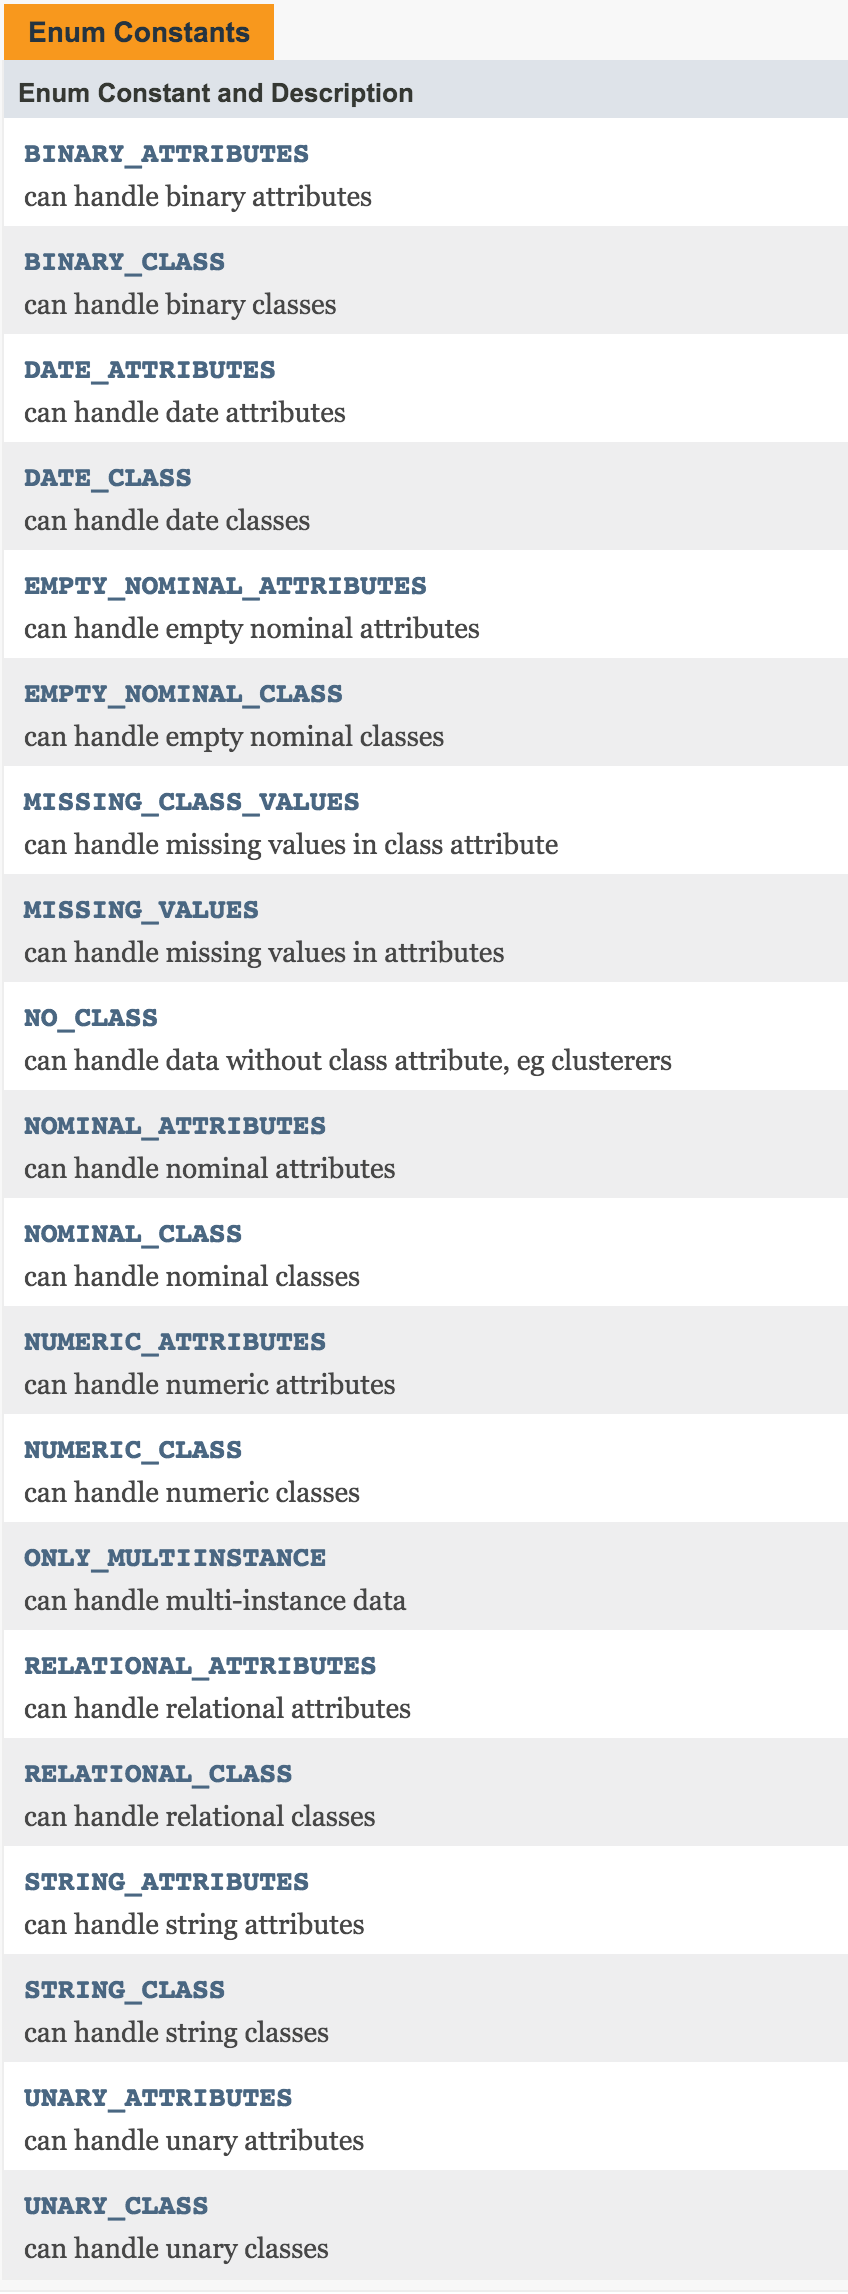
\includegraphics[width=0.6\textwidth]{images/B7_3.png}
\caption{Javadoc for the \textit{Capability} enumeration.}
\label{fig:javadoc_capability}
\end{figure}


In Figure~\ref{fig:scheme_id3}, \textit{Id3's} \textit{getCapabilities()} method first obtains a
\textit{Capabilities} object by calling \textit{super.getCapabilities()}. This returns a
\textit{Capabilities} object without any constraints. The best way to proceed
is to call the \textit{disableAll()} method on
the \textit{Capabilities} object and then enable the relevant
characteristics---those that the scheme can handle. \textit{Id3} does
just this, enabling the ability to handle nominal attributes, a
nominal class attribute and missing class values. It also specifies
that a minimum of zero training instances are required. For the most
part, individual capabilities are turned on or off by calling
the \textit{enable()} or \textit{disable()} method of
the \textit{Capabilities} object. These methods take constants that
are defined in the enumeration shown in
Figure~\ref{fig:javadoc_capability}, which is part of
the \textit{Capabilities} class.
